% !TEX encoding = UTF-8
% !TEX TS-program = pdflatex
% !TEX root = ../tesi.tex

%**************************************************************
\chapter{Realizzazione}
\label{cap:realizzazione}
%**************************************************************

\section{Pianificazione del lavoro}
In questa sezione verranno presentati i passaggi effettuati durante lo \textit{stage} per raggiungere un grado di comprensione sufficiente a produrre i risultati voluti. Partendo da uno studio delle tecnologie e dei concetti di base necessari ad avere un'idea del contesto in cui muoversi, passando quindi all'analisi dei \textit{framework} disponibili per realizzare gli obiettivi fissati, ed infine stilando una vera e propria lista di requisiti desiderabili.\\
Le sezioni riguardanti tecnologie e \textit{framework} saranno necessarie anche al lettore per comprendere appieno le scelte progettuali e di codifica effettuate.

\subsection{Studio delle tecnologie}
\subsubsection{Flutter}
E' impossibile parlare di Flutter senza prima discutere del linguaggio su cui si basa: Dart.\\
Faremo quindi un'introduzione quanto più sintetica possibile sulle sue caratteristiche più proprietarie, tralasciando invece le similitudini a linguaggi popolari che possono facilmente essere intuite dal lettore.\\
Dart è un linguaggio compilato fortemente tipizzato con sintassi simile a C, e adotta molte funzionalità tipiche dei linguaggi moderni: considera infatti ogni variabile un oggetto e implementa la \textit{null safety}, obbligando il programmatore a esplicitare con sintassi specifiche la presenza o meno del valore \verb+null+.

\begin{lstlisting}[language=dart, firstnumber=1,caption={Dart \textit{null safety}}]
    //dichiarazione di variabili
    String variabileNotNullable = '';  //non puo' mai essere null
    String? variabileNullable = null;  //puo' anche essere null

    //utilizzo esplicito di variabile nullable
    fun (variableNullable);   //compile error
    fun (?variableNullable);  //esplicito che puo' essere nulla

    //utilizzo esplicito di variabile not nullable
    if (value != null)
        fun (!value);   //dico al compilatore che sono certo value non sia null
\end{lstlisting} 

Permette inoltre l'interpolazione di stringhe:
\begin{lstlisting}[language=dart, firstnumber=1,caption={Dart interpolazone stringhe}]
    //sfrutto il simbolo $
    'number = $variableName';              //inserisco in stringa direttamente una variabile
    'expressionResult = ${expression}';    //inserisco in stringa direttamente un'espressione
\end{lstlisting}

Dart tratta in maniera particolare le funzioni, che sono oggetti, hanno un tipo (\verb+Function+), possono avere parametri posizioni o nominali, obbligatori od opzionali: 
\begin{lstlisting}[language=dart, firstnumber=1,caption={Dart parametri funzioni}]
    //parametri obbligatori posizionali
    void fun (int a, int b);  //non possono essere nulli, non essendo 'int? a'

    //possono essere anteceduti da parametri posizionali opzionali
    void fun (int a, int b, [String opz1 = '', String opz2 = '']){}
    void fun (int a, int b, [String? opz1nullable, String? opz2nullable]){}

    //oppure possono essere anteceduti da parametri nominali opzionali
    void fun (int a, int b, {String opz1 = '', String opz2 = ''}){}
    void fun (int a, int b, {String? opz1nullable, String? opz2nullable}){}

    //non possono essere anteceduti da entrambi
    void fun (int a, int b, [String opz1 = ''], {String opz2 = ''}){} //compile error

    //tutti i costruttori in Dart hanno solo parametri nominali
    //di default i parametri nominali sono opzionali
    //possono pero' essere resi obbligatori con la keyword 'required'
    void fun ({required String obb1, required String? obb2, String opz1 = ''}){}
\end{lstlisting}

Esistono le funzioni anonime (largamente sfruttate nei metodi \verb+build+ di Flutter), che possono essere ovviamente passate come argomento ad altre funzioni, essendo oggetti:
\begin{lstlisting}[language=dart, firstnumber=1,caption={Dart funzioni anonime}]
    //prima sintassi
    (){
        //corpo della funzione anonima
    } 

    //seconda sintassi
    () => return_expression

    //assegnamento di funzione anonima ad una variabile
    //ritorna una stringa con un messaggio portato in upper case
    var upperfy = (msg) => '${msg.toUpperCase()}';

    //passaggio di funzione come parametro
    fun (firstValue, () => secondValue);
\end{lstlisting}

Abbiamo delle espressioni condizionali specifiche del linguaggio dalla grande espressività e che quindi vengono largamente usate:
\begin{lstlisting}[language=dart, firstnumber=1,caption={Dart espressioni ternarie}]
    //primo tipo di condizione, detta ternaria
    condizione ? expr1 : expr2;

    //equivale a (in pseudocodice):
    if (condizione == true) return expr1
    else                    return expr2

    //vediamo un esempio
    int? a;               //a==null di default
    a = a==null ? 1 : 0;  //ad 'a' viene assegnato il valore 1 siccome a==null


    //################################
    //secondo tipo di condizione peculiare:
    expr1 ?? expr2;

    //equivale a (in pseudocodice):
    if (expr1 != null) return expr1
    else               return expr2

    //vediamo un esempio
    int? a;      //a==null di default
    a = a ?? 1;  //ad 'a' viene assegnato il valore 1 siccome a==null
\end{lstlisting}

I caratteri \verb+?+ e \verb+!+ sono, come si evince dalle espressioni ternarie e dalla \textit{null safety}, di cruciale importanza in Dart, ed è quindi opportuno vedere ancora qualche esempio del loro utilizzo:
\begin{lstlisting}[language=dart, firstnumber=1,caption={Dart operatori '?' e '!'}]
    list[1]     //accede al secondo elemento della lista

    list.?[1]
    //equivale a (in pseudocodice):
    if (list[1] != null)    return list[1]
    else                    return null

    //##############################

    foo?.bar 
    //equivale a (in pseudocodice):
    if (foo.bar != null)    return foo.bar
    else                    return null

    //##############################

    foo!.bar
    //equivale a (in pseudocodice):
    if (foo.bar != null)    return foo.bar
    else                    throw (runtimeException)
\end{lstlisting}

Le applicazioni \textit{mobile} e \textit{web} spesso si trovano a eseguire istruzioni che richiedono l'attesa di risorse esterne (ottenere dati dalla rete o leggerli da un \textit{file}, oppure scrivere su un \textit{database}). Per evitare il completo blocco dell'esecuzione (disastroso per un applicativo \textit{consumer}) Dart implementa nativamente delle funzioni di programmazione asincrona, che permetto di svolgere operazioni anche mentre altre sono in attesa.\\
Per fare ciò si serve di tre \textit{keyword}: \verb+async+, \verb+await+ e \verb+Future+:
\begin{lstlisting}[language=dart, firstnumber=1,caption={Dart operatori '?' e '!'}]
    Future<void> checkVersion () async {
        var version = await lookUpVersion();
    }

    //un'espressione marcata con la keyword 'await' ritorna sempre Future<T>
\end{lstlisting}

Trattiamo infine le caratteristiche peculiari di Dart per quanto riguarda classi e metodi:
\begin{itemize}
    \item Esistono i costruttori costanti, marcati \verb+const+, che sono inizializzati a \textit{compile-time}. Tutti gli altri sono implicitamente dinamici (quindi \textit{run-time});
    \item Posso creare costruttori nominati per implementare costruttori multipli tramite la sintassi:
\begin{lstlisting}[language=dart]
    ClassName.constructorName () :
        firstField = firstValue,
        secondField = secondValue;
\end{lstlisting}
    \item Ogni entità è una classe, ogni classe discende da \verb+Object+ (ad eccezione di \verb+Null+);
    \item Per ogni classe viene creata un'interfaccia implicita che contiene tutti i membri di istanza della classe;
    \item I metodi \textit{getter} e \textit{setter} di una classe vengono creati implicitamente per variabili non \verb+final+, ma possono essere definiti esplicitamente con le \textit{keyword} \verb+get+ e \verb+set+.
\end{itemize}

\subsubsection{Realtà aumentata}
\subsubsection{Ancoraggi in realtà aumentata}
\subsubsection{Azure Spatial Anchors}
\subsubsection{Gemello Digitale}

\subsection{Framework realtà aumentata per Flutter}
Essendo lo scopo di questo stage, e quindi il caso di studio di questa tesi, l'implementazione di una vista in realtà aumentata (nello specifico sfruttando asa) in un'applicazione preesistente sviluppata in Flutter, una grossa parte del lavoro svolto si è incentrato sullo studio dei framework e/o plug-in disponibili.\\
Sfortunatamente, complici la giovinezza di Flutter e la scarsa diffusione di tecnologie AR, le opzioni disponibili sono alquanto ridotte:
\begin{itemize}
    \item \textit{ar\_flutter\_plugin}: \href{https://pub.dev/packages/ar_flutter_plugin}{plugin} che punta a implementare le componenti AR in modalità cross-platform, quindi adattandosi autonomamente ad Android e iOS (sfruttando tuttavia le Cloud Anchor di Google). Nasce partendo da due plugin più specializzati: 
    \begin{itemize}
        \item \textit{arcore\_flutter\_plugin} (\href{https://github.com/giandifra/arcore_flutter_plugin}{Android});
        \item \textit{arkit\_flutter\_plugin} (\href{https://github.com/olexale/arkit_flutter_plugin}{iOS});
    \end{itemize}
    \item \textit{ARwayKit}: framework che mira a fornire un'integrazione semplificata, e in parte già completata, di una componente AR (ottenuta tramite asa) in Flutter tramite vista in Unity.
\end{itemize}
{\footnotesize Al momento della stesura di questo testo non è più possibile accedere liberamente alla \href{https://app.gitbook.com/s/-MCtct_TY9f3e8PrcV9T/arwaykit-with-flutter/quickstart-in-flutter}{documentazione} relativa ad ARwayKit, tuttavia è ancora reperibile un \href{https://medium.com/arway/building-ar-navigation-apps-with-flutter-and-arwaykit-280b69401cd9}{articolo} su \textit{medium.com} che ricalca la guida introduttiva precedentemente fornita dal sito ufficiale dell'azienda (è anche possibile trovarne una \href{https://web.archive.org/web/20220525060655/https://docs.arway.app/arwaykit-with-flutter/quickstart-in-flutter}{versione nella Wayback Machine}).}

\subsubsection{ARWayKit}
ARwayKit è un framework formato da un insieme di componenti che si pone l'obiettivo di fornire un'esperienza AR persistente, e lo persegue fornendo una SDK Unity, un'applicazione di Mapping e un insieme di API REST, che implementa le componenti AR in Flutter sfruttando \href{https://pub.dev/packages/flutter_unity_widget}{flutter\_unity\_widget}.\\
E' cross-platform, implementa le Anchor tramite asa e funziona in ambienti "gps-denied", ovvero dove i dati di posizone del gps non vengono utilizzati per muoversi all'interno dell'ambiente virtuale (oppure ambienti con protocolli di privacy elevati), il che lo rende apparentemente perfetto per il caso d'uso specifico di questa tesi, tuttavia presenta delle criticità: in primo luogo obbliga l'uso di Unity (sfruttando la sua caratteristica peculiare di poter essere importato come fosse una libreria) per sviluppare la vista AR, il che comporta non solo dover imparare il linguaggio ma dover anche configurare ulteriori componenti (come ad esempio \textit{Unity Hub}) che poi devono essere adottati assieme a quelli già in uso, appesantendo quindi il processo di codifica.\\
In secondo luogo troviamo invece il problema maggiore: la vista verrebbe realizzata nativamente in Unity, ovvero si tratta di una componente Unity separata rispetto all'applicazione che la lancia.
Questo renderebbe complesso se non impossibile usare dentro essa delle funzionalità Flutter: ad esempio, un bottone a schermo sarebbe un pulsante Unity, non Flutter, obbligando quindi poi a costruire una mappatura tra i due linguaggi per ogni funzionalità visualizzata.\\ 
Una vista così costruita non solo è scomoda da programmare, ma anche difficile da manutenere.\\

\begin{figure}[h!]
    \centering
    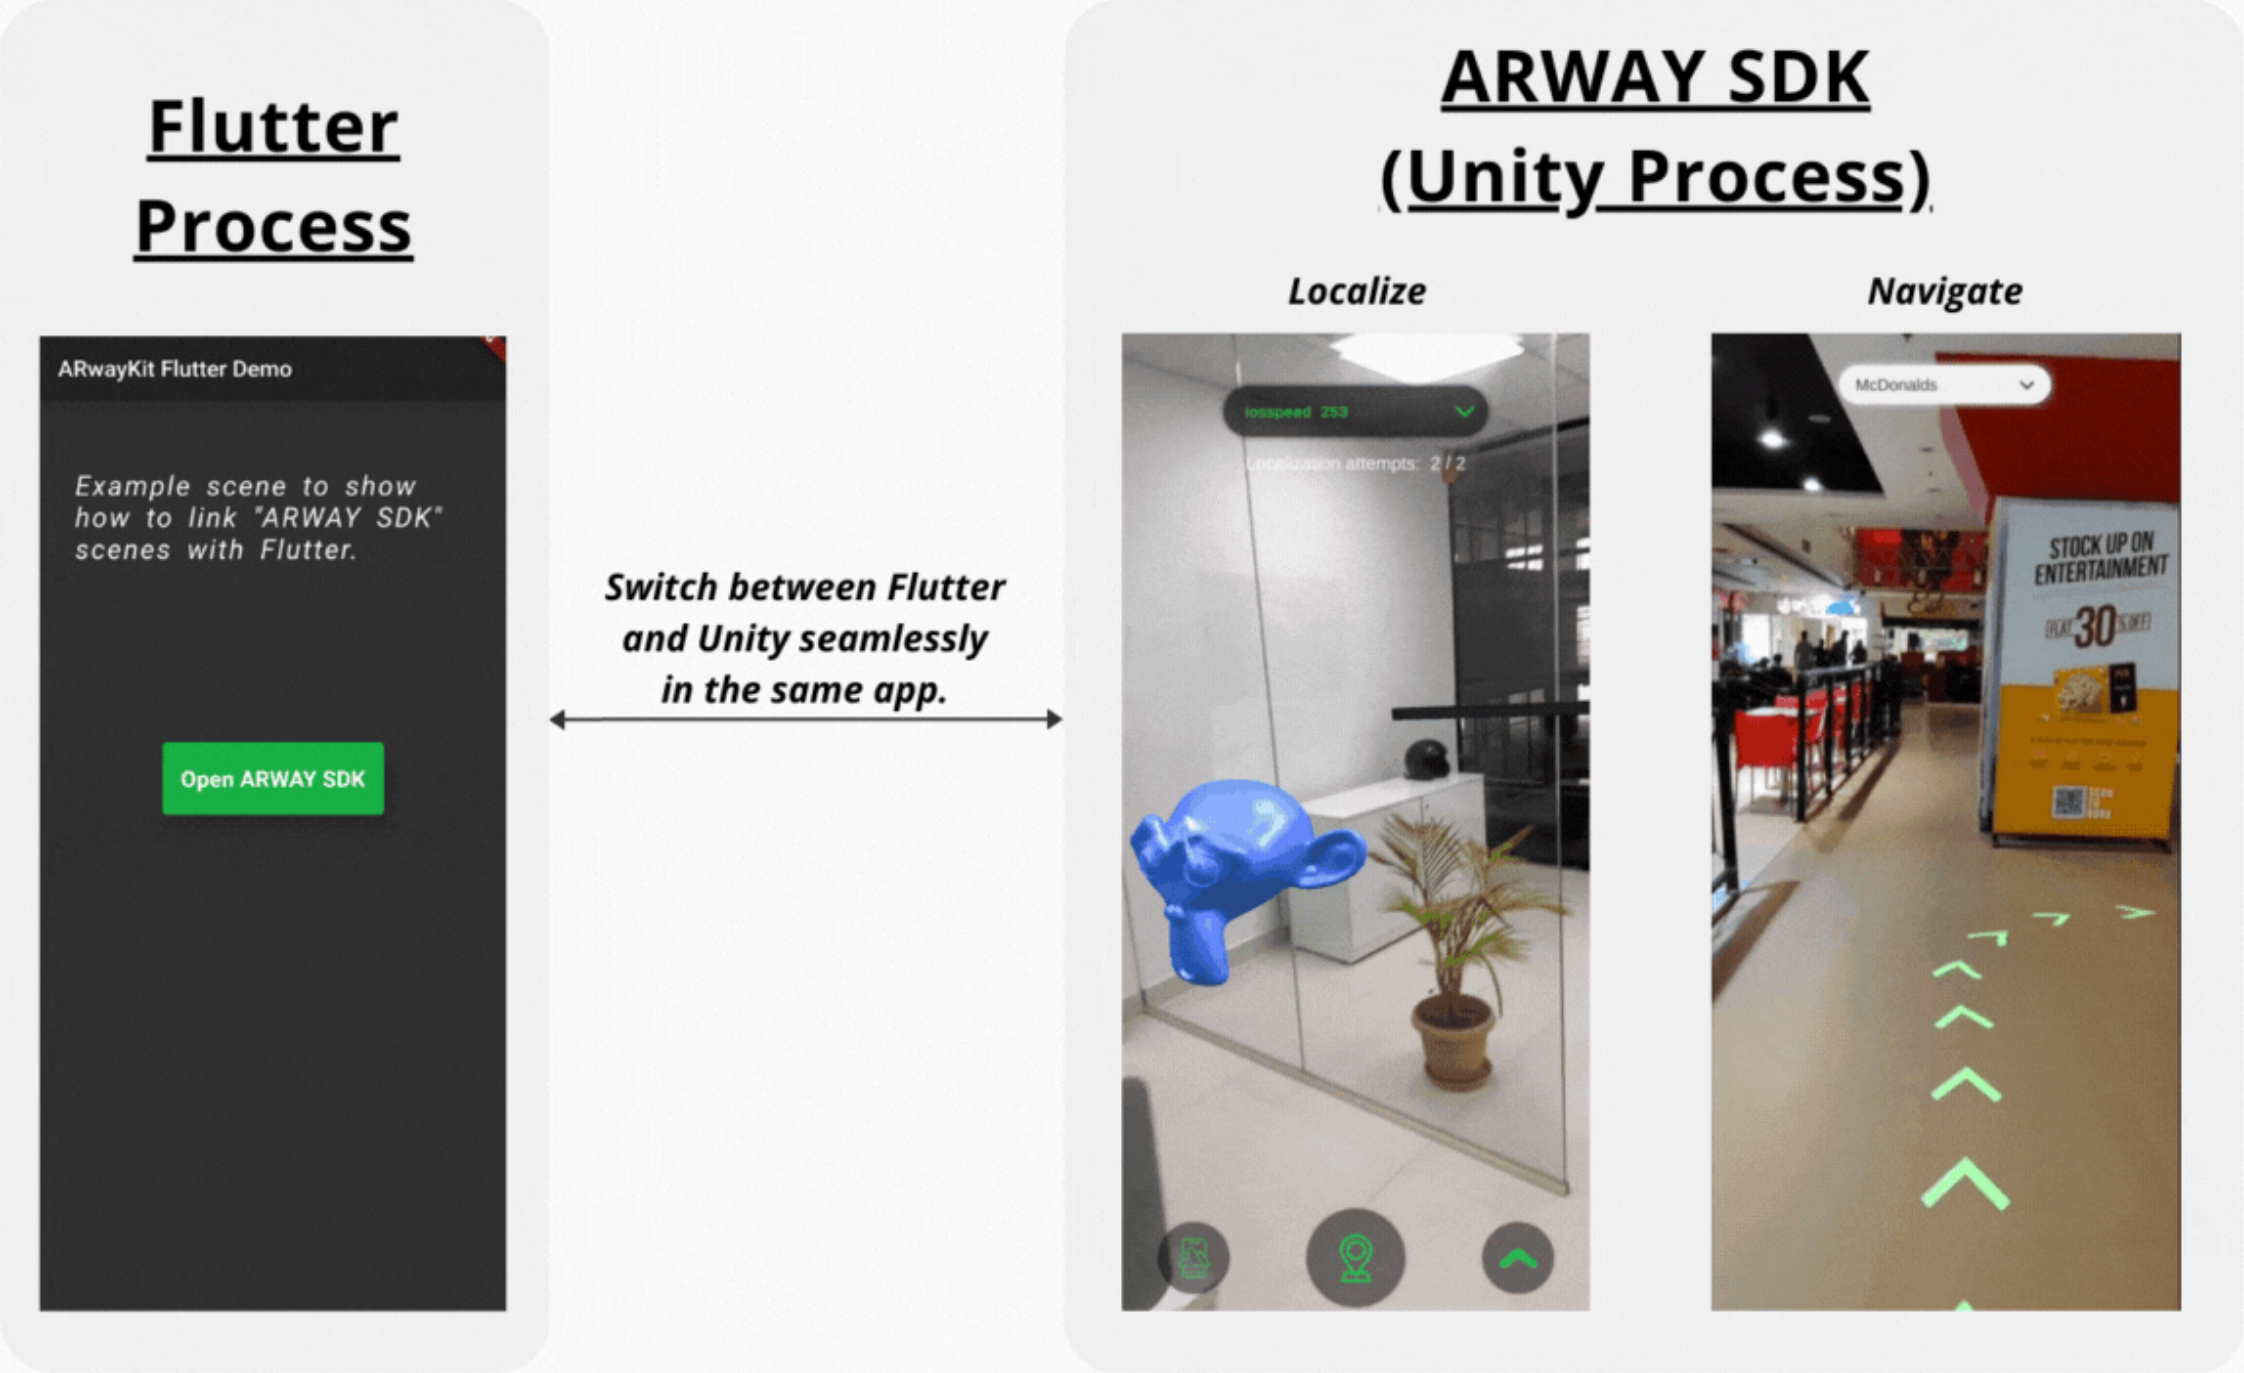
\includegraphics[height=5cm]{ARwayKit_samplegif_screenshot}
    \caption{Immagine esempio di utilizzo AR con ARwayKit}
\end{figure}

\subsubsection{ar\_flutter\_plugin}
\aplug{} è un plugin open source collaborativo estremamente giovane (il primo commit sulla repository pubblica risale al 6 febbraio 2021) che si pone l'obiettivo di implementare componenti in realtà aumentata in Flutter.\\
Per raggiungere lo scopo si serve della libreria archiviata \href{https://developers.google.com/sceneform/develop}{Sceneform}, che si occupa di "renderizzare scene 3D realistiche in applicazioni AR o meno, senza dover imparare OpenGL".\\
L'architettura di \aplug{} è composta da due parti: una API cross-platform unificata che fornisce un'interfaccia alle applicazioni tramite il plugin e le implementazioni specifiche per le piattaforme Android (in Kotlin) e iOS (in Swift) costruite su ARCore e ARKit rispettivamente, così da garantire accesso continuativo nel tempo a funzionalità aggiornate.\\
\aplug{} espone dei widget e delle classi 
\todo{}

\subsubsection{Confronto}

\subsection{Analisi dei requisiti}
Di seguito sono riportati i requisti individuati nel piano di lavoro proposto e a seguito di opportuni confronti con il tutor aziendale. Essi sono catalogati secondo la dicitura:
\begin{center}
    \textbf{R[Obbligatorietà][Tipologia][Codice]}
\end{center}
dove:
\begin{itemize}
    \item \textbf{Obbligatorietà}: specifica quanto un requisito sia vincolante per la riuscita del prodotto e può assumere i seguenti valori:
    \begin{itemize}
        \item \textbf{1: } Requisito obbligatorio;
        \item \textbf{2: } Requisito desiderabile ma non essenziale per il funzionamento;
        \item \textbf{3: } Requisito opzionale.
    \end{itemize}
    \item \textbf{Tipologia}: specifica la tipologia del requisito e può assumere i seguenti valori:
    \begin{itemize}
        \item \textbf{F: }\textit{funzionale,} determina una funzionalità necessaria all'applicazione;
        \item \textbf{V: }\textit{vincolo,} riguarda una caratteristica del prodotto decisa a monte.
    \end{itemize}
    \item \textbf{Codice}: identifica univocamente un requisito all'interno della sua tipologia (ovvero possono esistere due requisiti con lo stesso codice a patto che siano uno funzionale e uno di vincolo). Per i requisti subordinati si usa il "punto" come divisorio (\textit{ReqPadre, ReqPadre.Figlio1})
\end{itemize}

\subsubsection{Requisiti funzionali}
{
    \setlength{\freewidth}{\dimexpr\textwidth-10\tabcolsep}
    \renewcommand{\arraystretch}{1.5}
    \centering
    \setlength{\aboverulesep}{0pt}
    \setlength{\belowrulesep}{0pt}
    \rowcolors{2}{red!10}{white}
    \begin{longtable}{C{.15\freewidth} | C{1\freewidth}}
       \toprule
    \rowcolor{red}
    \textcolor{white}{\textbf{Codice}}&
    \textcolor{white}{\textbf{Descrizione}}\\
    \toprule
    \endhead

    R1F1 & Il plugin-in deve rappresentare asset tramite Anchor AR\\
    R1F2 & Il plugin-in deve rappresentare ticket tramite Anchor AR\\
    R1F3 & Il plug-in deve integrare le Anchor tramite asa\\
    R1F3.1 & Permettere aggiunta di asa\\%C
    R1F3.2 & Permettere recupero e visualizzazione di asa\\%R
    R2F3.3 & Permettere modifica di asa\\%U
    R1F3.4 & Permettere eliminazione di asa\\%D
    %API BACKEND
    R1F4 & Comunicare con Syn API\\
    R1F4.1 & Ricevere asset con Anchor associata\\
    R1F4.2 & Aggiungere asset con Anchor associata\\
    R2F4.3 & Ricevere ticket con Anchor associata\\
    R2F4.4 & Aggiungere ticket con Anchor associata\\
    %UI FLUTTER
    R1F5 & Utente deve poter vedere quali asset hanno anchor associata\\
    R2F6 & Utente deve poter vedere quali ticket hanno anchor associata\\
    R1F7 & Utente deve poter raggiungere l'anchor in vista AR dalla schermata dell'asset\\
    R1F8 & On-Tap su una anchor deve aprire una bottom sheet contestuale\\
    R1F8.1 & Bottom sheet deve presentare identificatore per asset o ticket associato alla anchor\\
    R1F8.2 & Bottom sheet associato a un asset mostra ultimi tre ticket aperti\\
    R1F8.3 & Bottom sheet deve fornire Call-To-Action per eliminare l'anchor\\
    R1F8.4 & Bottom sheet deve fornire Call-To-Action per raggiungere pagina di dettaglio\\
    R1F9 & Le informazioni contestuali di un ticket includono data e ora di creazione\\
    %UI AR
    R1F10 & Anchor hanno rappresentazione visiva contestuale\\ 
    R1F10.1 & Asset vengono rappresentati come \todo\\
    R1F10.2 & Ticket vengono rappresentati come \todo\\
    R1F11 & On-Tap sullo spazio permette di creare una Anchor in posizione\\
    R1F11.1 & Anchor posizionata nello spazio può essere salvata\\
    R1F11.2 & Anchor posizionata nello spazio può essere eliminata\\
    R1F12 & Il salvataggio di un'Anchor è disponibile solo quando è sicuro vada a buon fine\\
    R1F12.1 & Viene mostrato a schermo un feedback riguardo il livello di sicurezza raggiunto\\
    \bottomrule
    \rowcolor{white} 
    \caption{Tabella dei requisiti funzionali}
    \label{tab:requisiti-funzionali}
    \end{longtable}
}

\subsubsection{Requisiti di vincolo}
{
    \setlength{\freewidth}{\dimexpr\textwidth-10\tabcolsep}
    \renewcommand{\arraystretch}{1.5}
    \centering
    \setlength{\aboverulesep}{0pt}
    \setlength{\belowrulesep}{0pt}
    \rowcolors{2}{red!10}{white}
    \begin{longtable}{C{.15\freewidth} C{1\freewidth}} 
       \toprule
    \rowcolor{red}
    \textcolor{white}{\textbf{Codice}}&
    \textcolor{white}{\textbf{Descrizione}}\\
    \toprule
    \endhead

    R1V1 & Framework scelto funziona su Android\\
    R2V2 & Framework scelto funziona su iOS\\
    R1V3 & Framework scelto si integra con API Syn\\
    R1V3.1 & Framework ottiene con Anchor associata i dati degli asset\\
    R1V3.2 & Framework ottiene con Anchor associata i dati dei ticket\\
    R1V4 & Il framework scelto utilizza asa\\
    R1V5 & La vista AR deve essere sviluppata in Flutter\\
    \bottomrule
    \rowcolor{white} 
    \caption{Tabella dei requisiti di vincolo}
    \label{tab:requisiti-di-vincolo}
    \end{longtable}
}

\subsubsection{Riepilogo requisiti}
Sono stati individuati un totale di 36 requisiti, 29 funzionali e 7 di vincolo, di seguito schematizzati:
{
    \setlength{\freewidth}{\dimexpr\textwidth-10\tabcolsep}
    \renewcommand{\arraystretch}{1.5}
    \centering
    \setlength{\aboverulesep}{0pt}
    \setlength{\belowrulesep}{0pt}
    \rowcolors{2}{red!10}{white}
    \begin{longtable}{C{.25\freewidth} C{.2\freewidth}} 
       \toprule
    \rowcolor{red}
    \textcolor{white}{\textbf{Obbligatorietà}}&
    \textcolor{white}{\textbf{Quantità}}\\
    \toprule
    \endhead

    Obbligatori & 31\\
    Desiderabili & 5\\
    \bottomrule
    \rowcolor{white} 
    \caption{Numero di requisiti per obbligatorietà}
    \label{tab:requisiti-obbligatorieta}
    \end{longtable}
}

{
    \setlength{\freewidth}{\dimexpr\textwidth-10\tabcolsep}
    \renewcommand{\arraystretch}{1.5}
    \centering
    \setlength{\aboverulesep}{0pt}
    \setlength{\belowrulesep}{0pt}
    \rowcolors{2}{red!10}{white}
    \begin{longtable}{C{.25\freewidth} C{.2\freewidth}} 
       \toprule
    \rowcolor{red}
    \textcolor{white}{\textbf{Tipologia}}&
    \textcolor{white}{\textbf{Quantità}}\\
    \toprule
    \endhead

    Funzionali & 29\\
    Di Vincolo & 7\\
    \bottomrule
    \rowcolor{white} 
    \caption{Numero di requisiti per tipologia}
    \label{tab:requisiti-tipolgia}
    \end{longtable}
}

\subsection{Attività di supporto}
\subsubsection{Interazione aziendale}
\subsubsection{Processi di verifica e validazione}
%************************************************************************************************************
\section{Difficoltà incontrate}
\subsection{Problemi documentali}
\subsection{Problemi tecnologici}

%************************************************************************************************************

\section{Risultati raggiunti}
\subsection{Copertura requisiti}
\subsection{Implementazione Android}
\subsection{Implementazione iOS}
